\documentclass[landscape,a0paper,fontscale=0.292]{baposter}

\usepackage[vlined]{algorithm2e}
\usepackage{times}
\usepackage{calc}
\usepackage{url}
\usepackage{graphicx}
\usepackage{amsmath}
\usepackage{amssymb}
\usepackage{relsize}
\usepackage{multirow}
\usepackage{booktabs}
\usepackage{makecell}
\usepackage{threeparttable}
\usepackage{subfig}
\usepackage{graphbox}
\usepackage{wrapfig}

\usepackage{multicol}
\usepackage[T1]{fontenc}
\usepackage{ae}
\usepackage{enumitem}
\newcommand\Tstrut{\rule{0pt}{2.2ex}}       % "top" strut
\newcommand\Bstrut{\rule[-1ex]{0pt}{0pt}} % "bottom" strut
\newcommand{\TBstrut}{\Tstrut\Bstrut} % top&bottom struts
\newcommand{\padl}{\hspace{1pt}}
\newcommand{\padr}{\hspace{1pt}}

\usepackage{colortbl}
\usepackage{xcolor}

\definecolor{ctitle}{HTML}{2c2739}
\definecolor{mypurple}{HTML}{d2cce1}

\usepackage[pagebackref=true,breaklinks=true,colorlinks=true,bookmarks=false,linkcolor={red!50!black},urlcolor={magenta},citecolor={green!50!black}]{hyperref} 

\setlist[itemize]{leftmargin=*,nosep}
    \setlength{\columnsep}{0.7em}
    \setlength{\columnseprule}{0mm}

\setlist[enumerate]{leftmargin=2.5em,nosep}
    \setlength{\columnsep}{1.0em}
    \setlength{\columnseprule}{0mm}

%%%%%% abbreviations
\makeatletter
\DeclareRobustCommand\onedot{\futurelet\@let@token\@onedot}
\def\@onedot{\ifx\@let@token.\else.\null\fi\xspace}

\def\eg{\emph{e.g}\onedot} \def\Eg{\emph{E.g}\onedot}
\def\ie{\emph{i.e}\onedot} \def\Ie{\emph{I.e}\onedot}
\def\cf{\emph{c.f}\onedot} \def\Cf{\emph{C.f}\onedot}
\def\etc{\emph{etc}\onedot} \def\vs{\emph{vs}\onedot}
\def\wrt{w.r.t\onedot} \def\dof{d.o.f\onedot}
\def\etal{\emph{et al}\onedot}
\makeatother

% %%%%%%%%%%%%%%%%%%%%%%%%%%%%%%%%%%%%%%%%%%%%%%%%%%%%%%%%%%%%%%%%%%%%%%%%%%%%%%%%
% % Save space in lists. Use this after the opening of the list
% %%%%%%%%%%%%%%%%%%%%%%%%%%%%%%%%%%%%%%%%%%%%%%%%%%%%%%%%%%%%%%%%%%%%%%%%%%%%%%%%
% \newcommand{\compresslist}{%
% \setlength{\itemsep}{0pt}%
% \setlength{\itemsep}{0pt}%
% \setlength{\parskip}{0pt}%
% \setlength{\parsep}{0pt}%
% }
\renewcommand{\rmdefault}{ptm} % Arial
\renewcommand{\sfdefault}{ptm} % Arial

\newcommand{\viewdir}{\boldsymbol{d}}
\newcommand{\lightloc}{\boldsymbol{p}_l}
\newcommand{\lightint}{L_e}
\newcommand{\ray}{\boldsymbol{r}}
\newcommand{\pixelcolor}{\boldsymbol{C}}
\newcommand{\loss}{\mathcal{L}}
\newcommand{\point}{\boldsymbol{x}}
\newcommand{\lin}{L_{int}}
\newcommand{\din}{\boldsymbol{w}_i}
\newcommand{\normal}{\boldsymbol{n}}
\newcommand{\brdf}{f_m}

%%%%%%%%%%%%%%%%%%%%%%%%%%%%%%%%%%%%%%%%%%%%%%%%%%%%%%%%%%%%%%%%%%%%%%%%%%%%%
%% Begin of Document
%%%%%%%%%%%%%%%%%%%%%%%%%%%%%%%%%%%%%%%%%%%%%%%%%%%%%%%%%%%%%%%%%%%%%%%%%%%%%
\begin{document}
%%%%%%%%%%%%%%%%%%%%%%%%%%%%%%%%%%%%%%%%%%%%%%%%%%%%%%%%%%%%%%%%%%%%%%%%%%%%%
%% Here starts the poster
%%---------------------------------------------------------------------------
%% Format it to your taste with the options
%%%%%%%%%%%%%%%%%%%%%%%%%%%%%%%%%%%%%%%%%%%%%%%%%%%%%%%%%%%%%%%%%%%%%%%%%%%%%
\begin{poster}{
    % Show grid to help with alignment
    grid=false,
    columns=6,
    % Column spacing
    colspacing=0.7em,
    % Color style
    headerColorOne=mypurple,
    borderColor=mypurple,
    % Format of textbox
    textborder=faded,
    % Format of text header
    headerborder=open,
    headershape=roundedright,
    headershade=plain,
    background=none,
    bgColorOne=cyan!10!white,
    headerheight=0.17\textheight
}
% Eye Catcher
{
    \raisebox{0.075\height}{
\includegraphics[height=0.0445\linewidth]{logo/HKU}}
    \makebox[0.005\textwidth]{} 
    \raisebox{0.075\height}{
\includegraphics[height=0.0445\linewidth]{logo/cuhksz}}
    \makebox[0.005\textwidth]{} 
    \raisebox{0.075\height}{
\includegraphics[height=0.0445\linewidth]{logo/NTU}}
    \makebox[0.005\textwidth]{} 
    \raisebox{0.075\height}{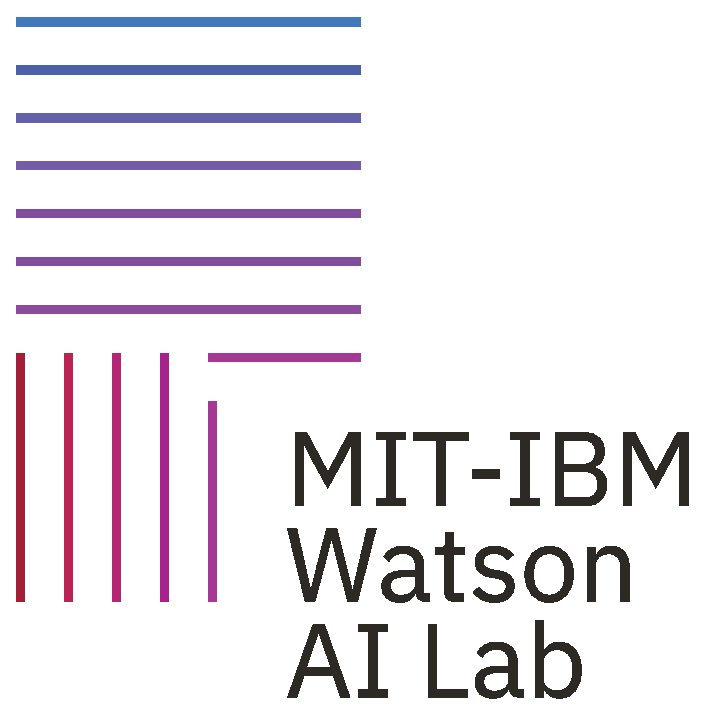
\includegraphics[height=0.0445\linewidth]{logo/MIT-IBM}}
}
% Title
{
    \\[0.3em]\sc\huge\bf \textcolor{ctitle}{\Huge{S$^3$-NeRF}}: Neural Reflectance Field from \textcolor{ctitle}{\Huge{S}}hading and \textcolor{ctitle}{\Huge{S}}hadow\\[0.15em] under a \textcolor{ctitle}{\Huge{S}}ingle Viewpoint
}
% Authors
{
    \vspace{0.3em} Wenqi Yang$^1$ \enspace Guanying Chen$^2$ \enspace Chaofeng Chen$^3$ \enspace Zhenfang Chen$^4$ \enspace Kwan-Yee K. Wong$^1$ \\[0.2em]
    {$^1$The University of Hong Kong \enspace$^2$FNii and SSE, CUHK-Shenzhen \\[0.1em] $^3$Nanyang Technological University \enspace$^4$MIT-IBM Watson AI Lab}
}
% University logo
{
    \begin{tabular}{c}
        \raisebox{-0.9\height}{
\includegraphics[align=c,width=0.14\linewidth]{logo/nips}}\\[0.5em]
        \raisebox{-0.5\height}{
        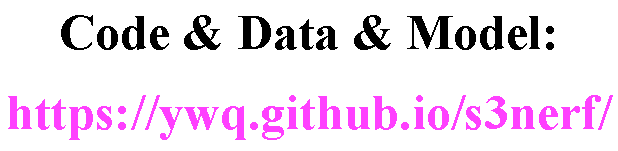
\includegraphics[align=c,width=0.12\linewidth]{logo/link.pdf}\hspace{0.002\linewidth}
        
\includegraphics[align=c,height=0.05\linewidth]{logo/qr_code.png}}
    \end{tabular}
}

%%%%%%%%%%%%%%%%%%%%%%%%%%%%%%%%%%%%%%%%%%%%%%%%%%%%%%%%%%%%%%%%%%%%%%%%%%%%%%
%%% Now define the boxes that make up the poster
%%%---------------------------------------------------------------------------
%%% Each box has a name and can be placed absolutely or relatively.
%%% The only inconvenience is that you can only specify a relative position 
%%% towards an already declared box. So if you have a box attached to the 
%%% bottom, one to the top and a third one which should be inbetween, you 
%%% have to specify the top and bottom boxes before you specify the middle 
%%% box.
%%%%%%%%%%%%%%%%%%%%%%%%%%%%%%%%%%%%%%%%%%%%%%%%%%%%%%%%%%%%%%%%%%%%%%%%%%%%%%

%%%%%%%%%%%%%%%%%%%%%%%%%%%%%%%%%%%%%%%%%%%%%%%%%%%%%%%%%%%%%%%%%%%%%%%%%%%%%%
\headerbox{\bf\color{ctitle} Idea}{name=idea,column=0,row=0,span=2}{
    \begin{minipage}[c]{\textwidth}
        \begin{itemize}
            \item ``Dual problem'' of Multi-View Scene reconstruction -- utilize {\bf single-view} images captured under {\bf different point lights} to reconstruct a scene. 
            \item Existing single-view methods -- only recover a \textbf{2.5D} scene representation (\ie, a normal / depth map for the visible surface). 
            \item Ours -- Learn a \textbf{3D} neural reflectance field. 
            \item MVS -- Rely on multi-view photo-consistency to infer scene geometry.
            \item Ours -- Exploit two information-rich monocular cues -- \textbf{shading} \& \textbf{shadow}.
        \end{itemize} 
    \end{minipage}
}
\headerbox{\bf\color{ctitle} Overview}{name=contribution,column=2,row=0,span=4}{
    \begin{minipage}[c]{0.4\textwidth}
        \textbf{\color{ctitle}Contributions:}
        \vspace{0.2em}
        \begin{itemize}
            \item Novel problem: 3D neural reflectance field optimization from single-view images captured under different point lights.
            \item Exploit monocular shading and shadow cues to jointly recover the geometry and BRDFs of a scene.
            \item Adopt an efficient online shadow computation to fully exploit the information-rich shading and shadow cues.
            \item Experiments on multiple challenging datasets show that S$^3$-NeRF can faithfully reconstruct a complete scene geometry from single-view images and is robust to depth discontinuity.
        \end{itemize}  
    \end{minipage}\hfill
    \begin{minipage}[c]{0.6\textwidth}
        \begin{center}
            \hfill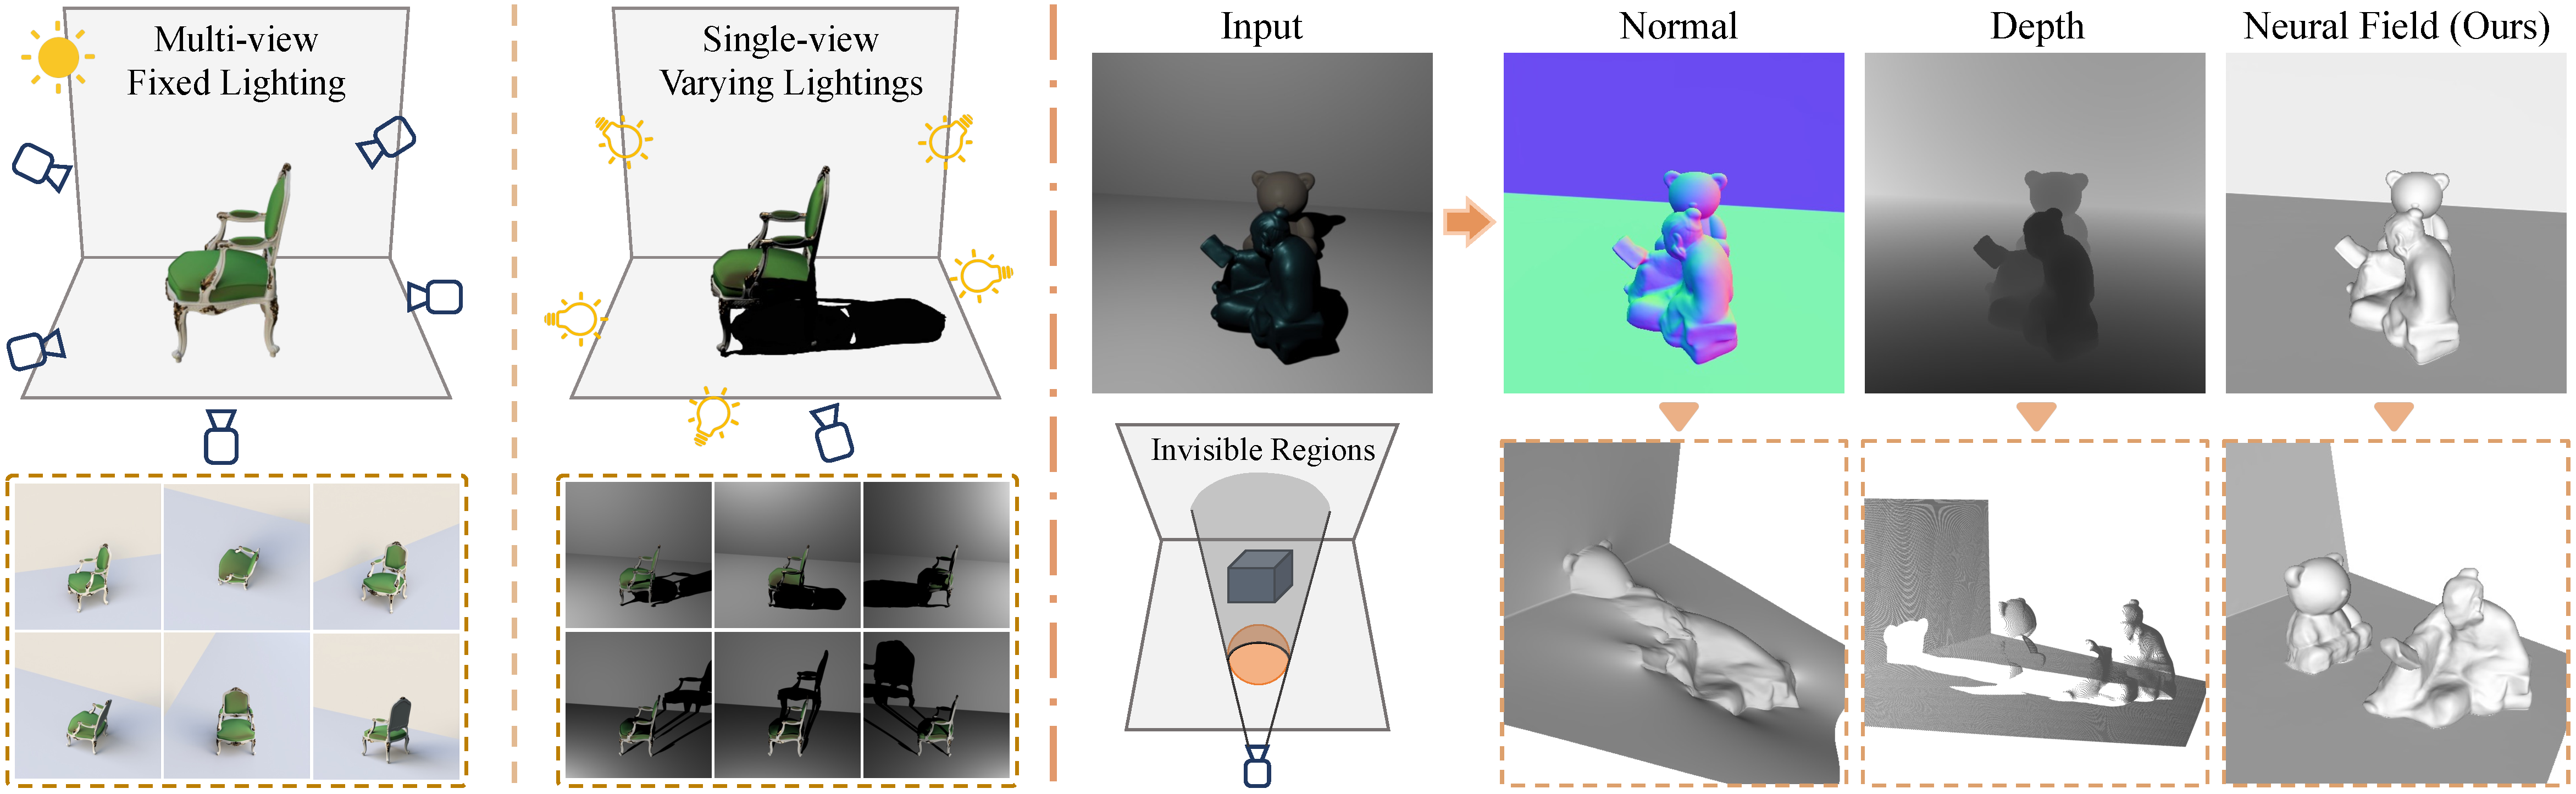
\includegraphics[width=0.98\textwidth]{images/intro.pdf}\\
            \vspace{-0.2em}
            \makebox[0.4\textwidth]{\footnotesize (a) Different capturing setups}
            \makebox[0.59\textwidth]{\footnotesize (b) Comparison of different scene representations}
        \end{center}
         
    \end{minipage}
}

\headerbox{\bf\color{ctitle} Method}{name=method,column=0,below=idea,span=2}{
    \textbf{\color{ctitle}Overview:} \\
    Given $N$ images captured from a single viewpoint under different near point lights, S$^3$-NeRF targets at recovering the geometry and materials of the scene.
    \vspace{-1.5em}
    \begin{center}
        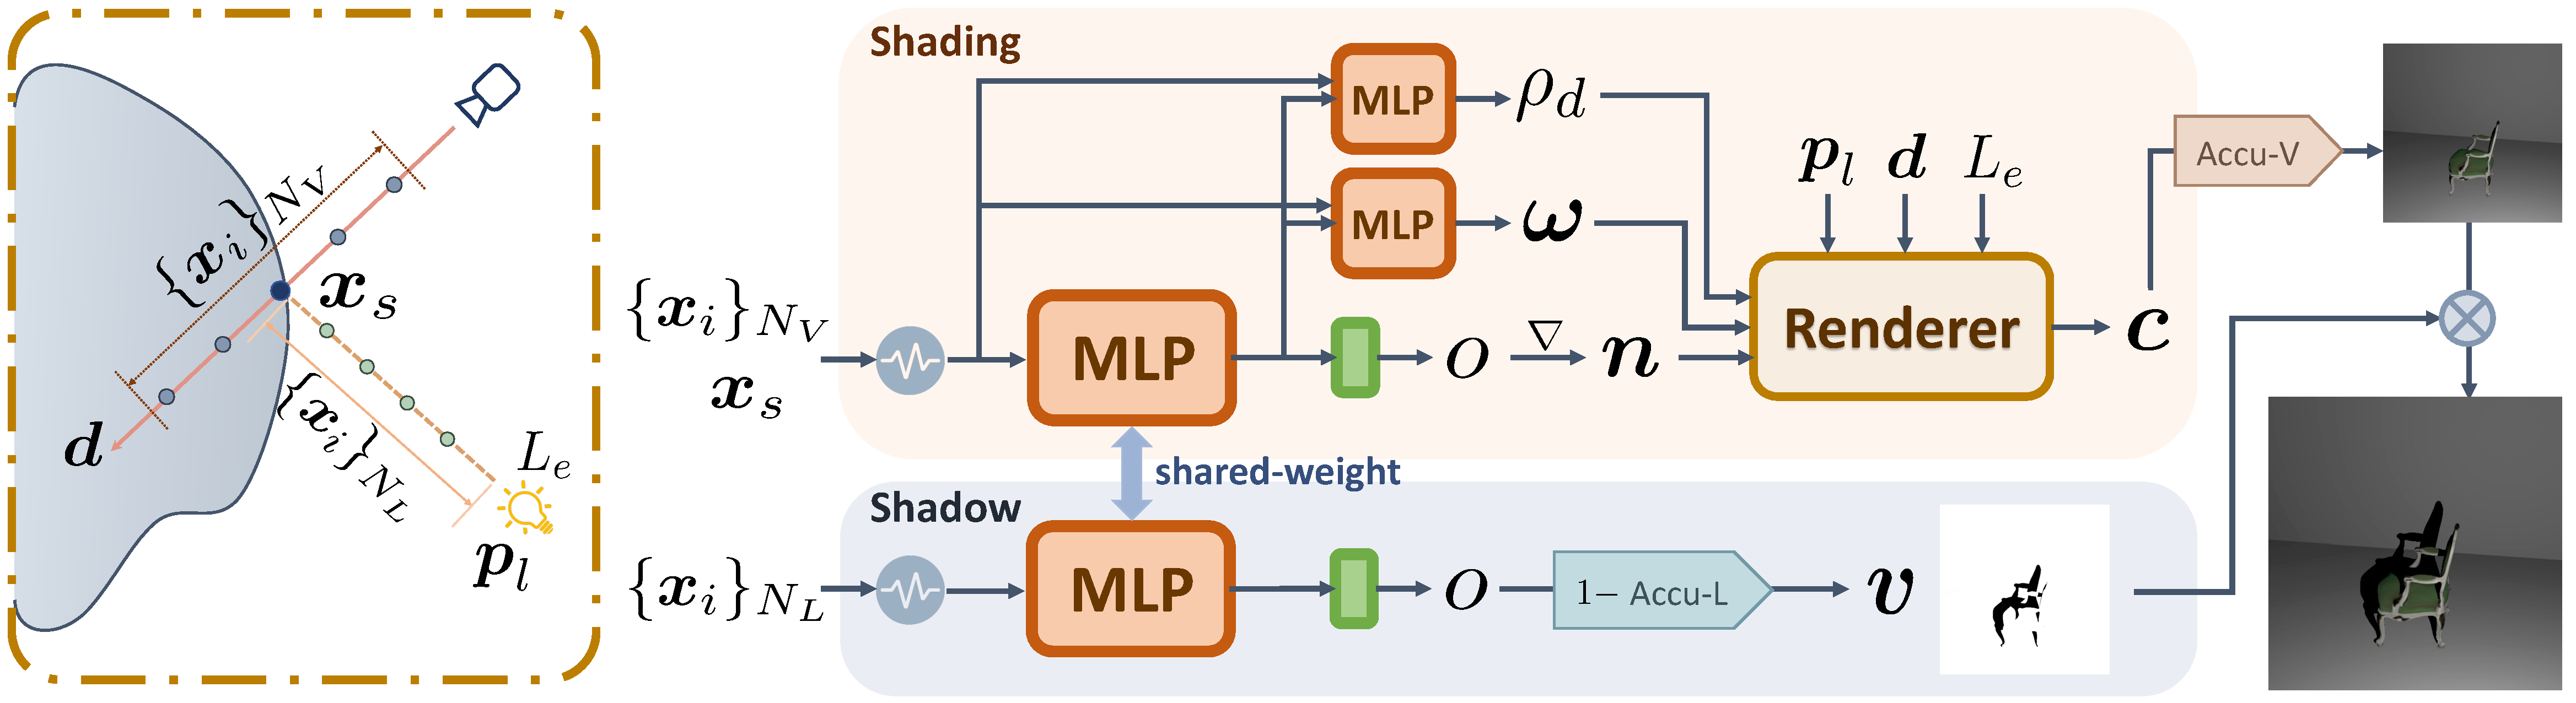
\includegraphics[width=\textwidth]{images/method_v2.pdf}
    \end{center}
    \vspace{-0.8em}
    We first apply root-finding to locate the surface intersection point $\point_s$. 
    \begin{itemize}
        \item $N_V$ points on the camera ray are sampled around the surface to generate accumulated shading values. 
        \item $N_L$ points are sampled on the surface-to-light segment to calculate the light visibility ($O(N_L)$ MLP queries per ray, calculated in an online manner). 
    \end{itemize}
    
    \vspace{0.5em}
    \textbf{\color{ctitle}Rendering Model:}  \\[0.2em]
    We consider non-Lambertian surfaces with spatially-varying BRDFs. The rendering equation for a surface point $\point$ viewed from a direction $\viewdir$ under a near point light $(\lightloc, \lightint)$ can be written as
    \vspace{-0.5em}
    {\small
    \begin{align*}
        f_c(\viewdir, \lightloc, \lightint ; \point) 
        &= \underbrace{\lin(\lightloc, \lightint; \point)}_{\text{Light Intensity}} \underbrace{\brdf (\viewdir, \din(\lightloc;\point); \point)}_{\text{BRDF Value}} \underbrace{\max\left(\din(\lightloc;\point) \cdot \normal(\point), 0 \right)}_{\text{Shading}}.
    \end{align*}
    }
    \vspace{-1em}\\
    We propose to adopt a joint volume and surface rendering strategy:
    \vspace{-0.8em}
    {\small
    \begin{align*}
        \pixelcolor_v(\ray)&= f_v(\lightloc; \point_{s}) \sum_{i=1}^{N_V} o(\point_{i}) \prod_{j<i}\left(1-o\left(\point_{j}\right)\right)  f_c(\point_{i}, \viewdir, \lightloc, \lightint ), \\
        \pixelcolor_s(\ray) &= f_v(\lightloc; \point_{s})f_c( \viewdir, \lightloc, \lightint ;\point_{s}).
    \end{align*}
    }
    \vspace{-1.2em}
    
    \vspace{0.2em}
    \begin{minipage}[c]{0.54\textwidth}
    \textbf{\color{ctitle}Alternative Shadow Modeling:} 
    \vspace{0.2em}
        \begin{enumerate}[leftmargin=*,nosep,label={(\alph*)}]
            \item Calculate light visibilities for all $N_V$ points sampled along the ray (computationally expensive).
            \item Adopt an MLP to directly regress light visibility of a point to reduce the queries for each ray.
        \end{enumerate}
    \end{minipage}
    \hfill
    \begin{minipage}[c]{0.45\textwidth}
    \begin{center}
        \hfill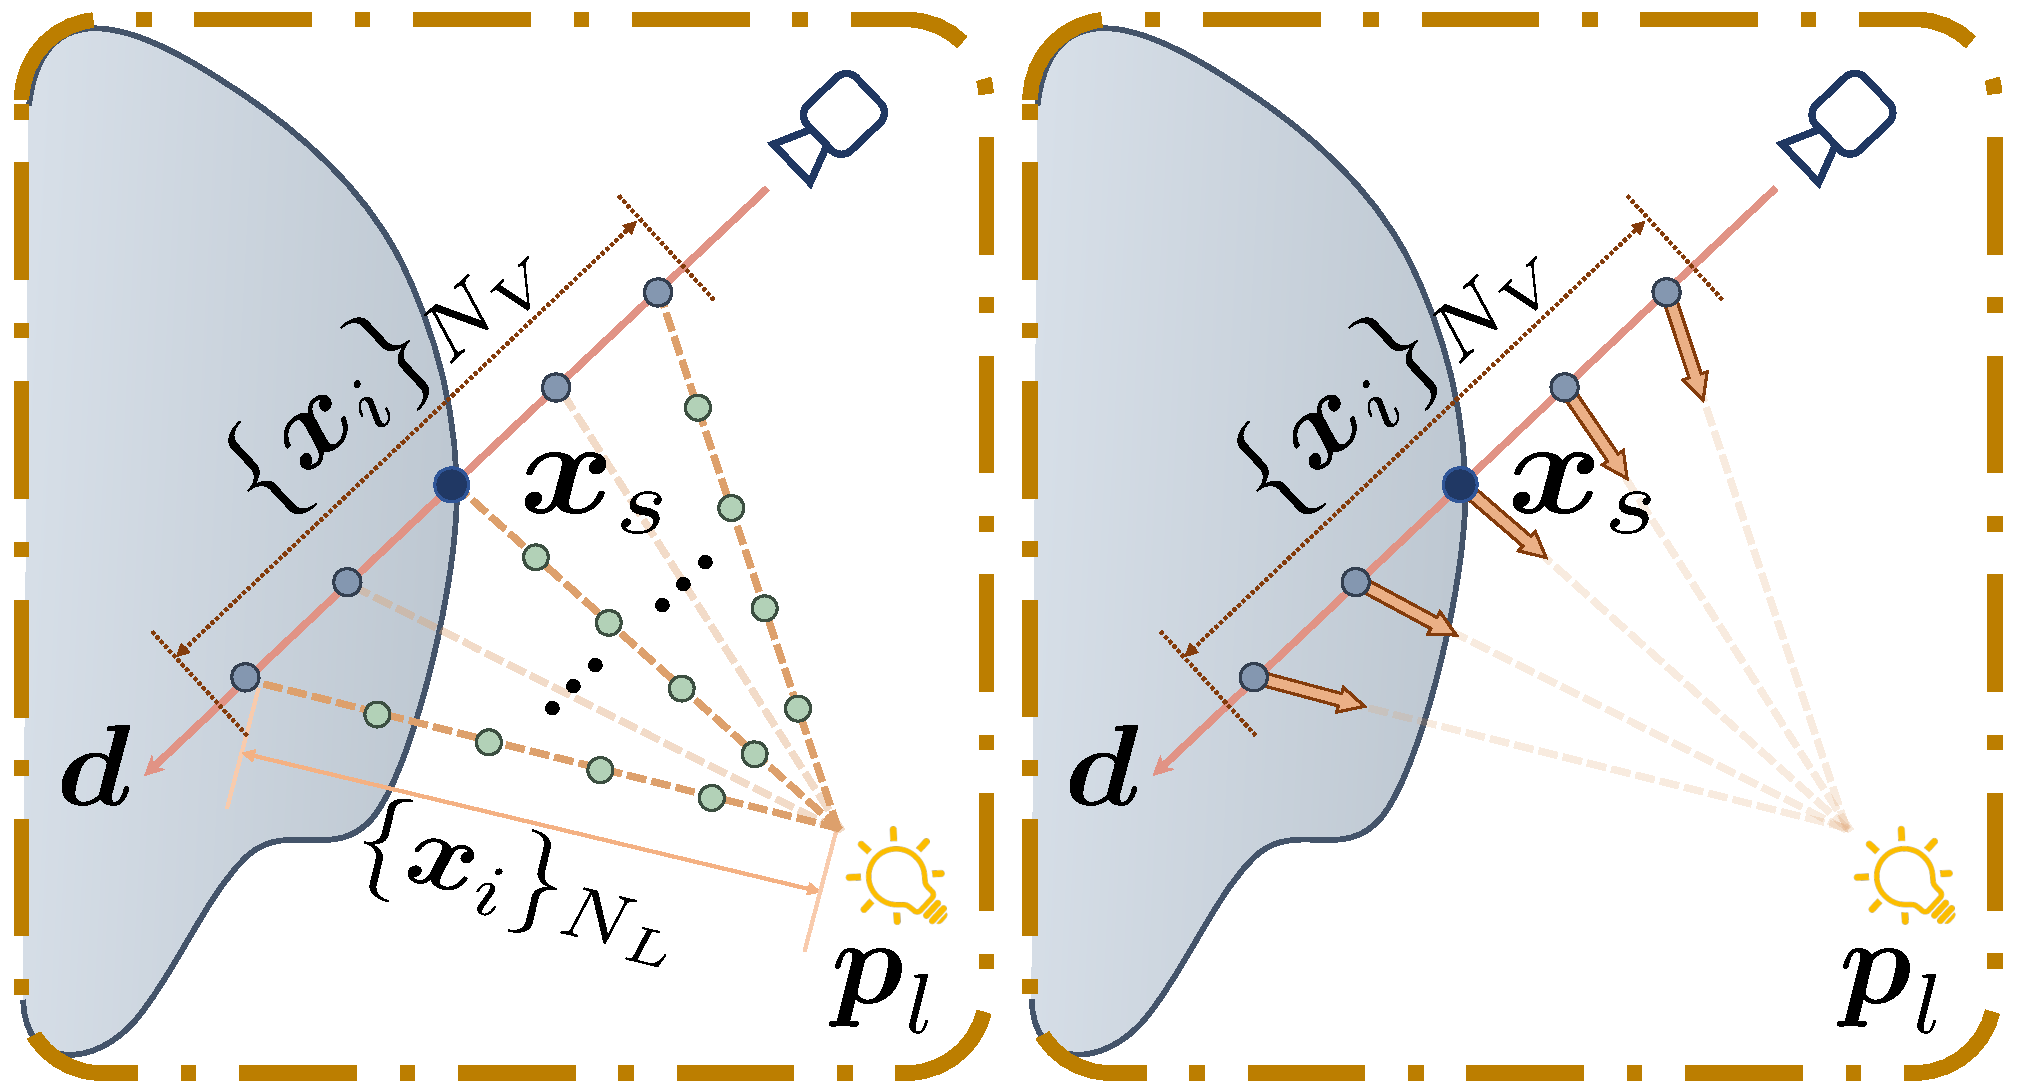
\includegraphics[width=0.98\textwidth]{images/shadow.pdf}\\
        \vspace{-0.3em}
        \makebox[0.49\textwidth]{\footnotesize (a) $O(N_VN_L)$}
        \makebox[0.49\textwidth]{\footnotesize (b) $O(N_V)$} \\
    \end{center}
    \end{minipage}
    
}
%
\headerbox{\bf\color{ctitle} Experiments \& Results}{name=results,column=2,below=contribution,span=4}{
    \begin{minipage}[t]{0.49\textwidth}
        %%%%%%%%%%%%%%%%%%% Neural Radiance Field  %%%%%%%%%%%%%%%%%%%%%%
        \textbf{\color{ctitle}Comparison with Neural Radiance Field Methods:}
        %%%%%%%%%%%%%%%%%%%%%%%% table  %%%%%%%%%%%%%%%%%%%%%%%%%%%%%
        \vspace{-0.8em}
        \begin{center}
            Quantitative results on relighting and normal estimation\\
            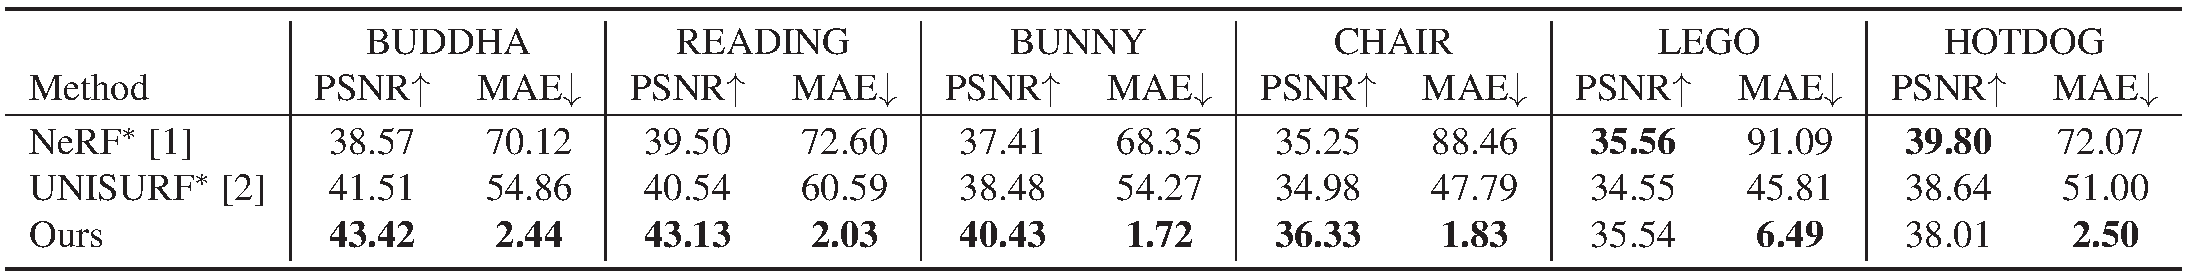
\includegraphics[width=\textwidth]{images/table_baseline_nerf.pdf}
        \end{center}
        \vspace{-2em}
        %%%%%%%%%%%%%%%%%%%%%%%% figure  %%%%%%%%%%%%%%%%%%%%%%%%%%%%%
        \begin{center}
            Qualitative results on relighting and normal estimation \\
            \includegraphics[width=\textwidth]{images/fig_baseline_nerf.pdf}
        \end{center}
        
        \vspace{-0.6em}
        %%%%%%%%%%%%%%%%%%%%%%%% Single-view  %%%%%%%%%%%%%%%%%%%%%%%%%
        \textbf{\color{ctitle}Comparison with Single-view Shape Estimation Methods:}
        %%%%%%%%%%%%%%%%%%%%%%%% table  %%%%%%%%%%%%%%%%%%%%%%%%%%%%%
        \vspace{-0.7em}
        \begin{center}
            Quantitative comparison (only object regions)\\
            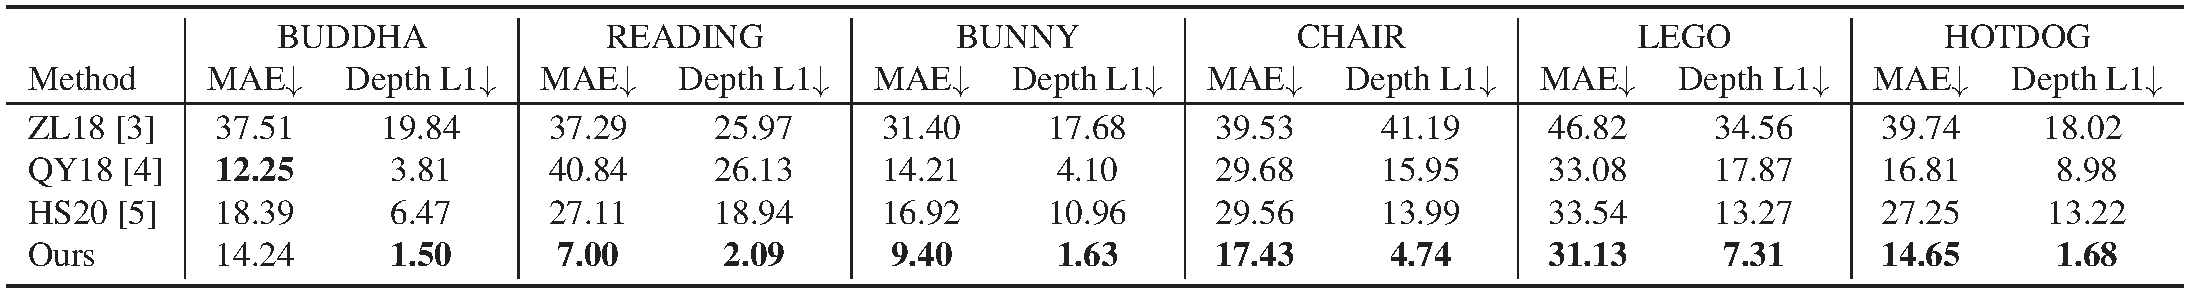
\includegraphics[width=\textwidth]{images/table_baseline_ps.pdf}
        \end{center}
        \vspace{-1.8em}
        %%%%%%%%%%%%%%%%%%%%%%%% figure  %%%%%%%%%%%%%%%%%%%%%%%%%%%%%
        \begin{center}
            Qualitative comparison with single-view normal / depth estimation baselines \\
            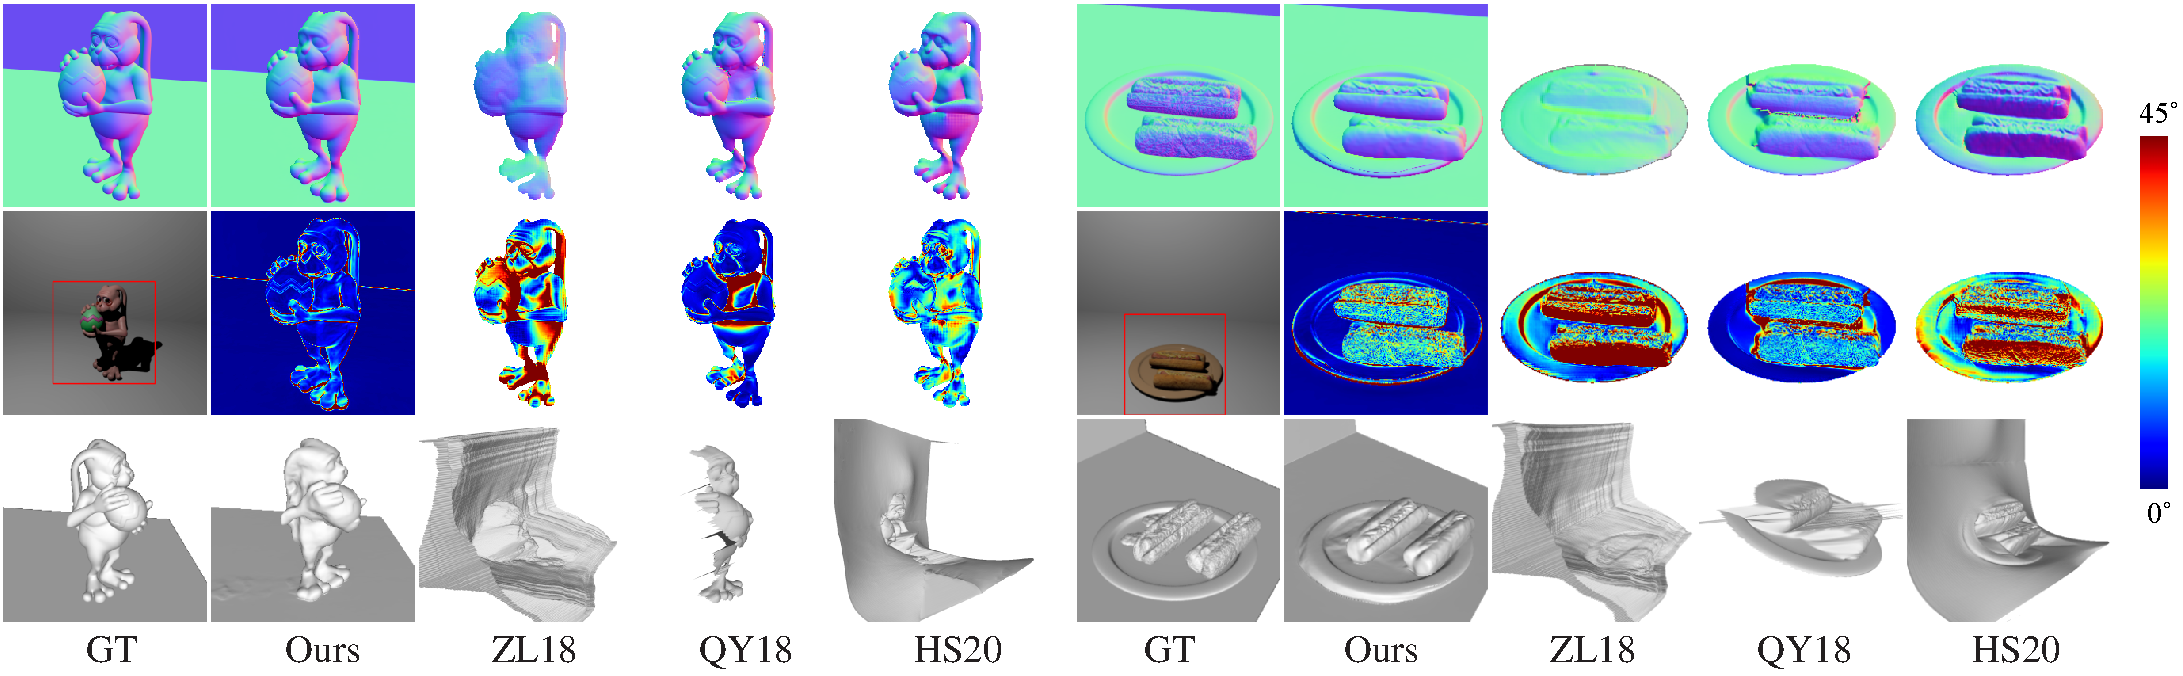
\includegraphics[width=\textwidth]{images/fig_baseline_ps.pdf} 
        \end{center}
    \end{minipage}\hfill
    %%%%%%%%%%%%%%%%%%%%%%%%%%%%%%%%%%%%%%%%%%%%%%%%%%%%%%%%%%%%%%%%%%
    %%%%%%%%%%%%%%%%% second column %%%%%%%%%%%%%%%%%%%%%%%%%%%%%%%%%%
    %%%%%%%%%%%%%%%%%%%%%%%%%%%%%%%%%%%%%%%%%%%%%%%%%%%%%%%%%%%%%%%%%%
    \begin{minipage}[t]{0.49\textwidth}
        %%%%%%%%%%%%%%%%%%%%%%%% Ablation  %%%%%%%%%%%%%%%%%%%%%%%%%%%%
        \textbf{\color{ctitle}Ablation Study:} 
        %%%%%%%%%%%%%%%%%%%%%%%% table  %%%%%%%%%%%%%%%%%%%%%%%%%%%%%
        \vspace{-0.8em}
        \begin{center}
            Quantitative results for the ablation study\\
            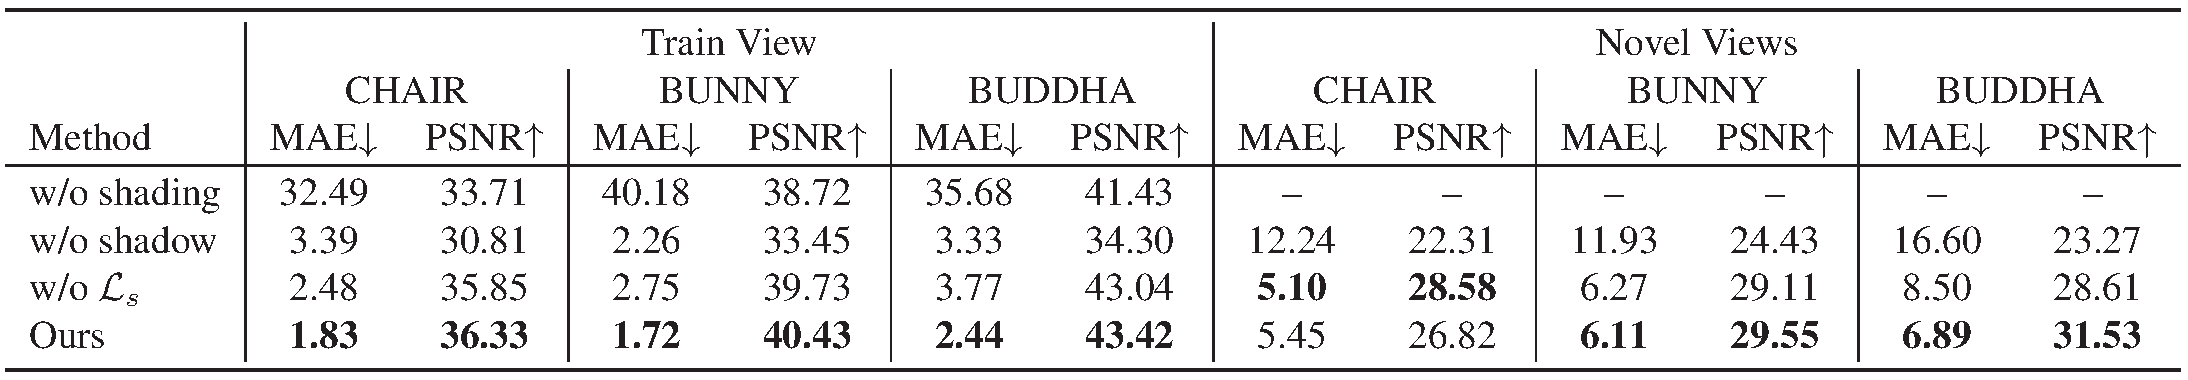
\includegraphics[align=c,width=\textwidth]{images/table_ablation.pdf} 
        \end{center}
        \vspace{-1.6em}
        %%%%%%%%%%%%%%%%%%%%%%%% figure  %%%%%%%%%%%%%%%%%%%%%%%%%%%%%
        \begin{center}
            Visual results for the ablation study \\
            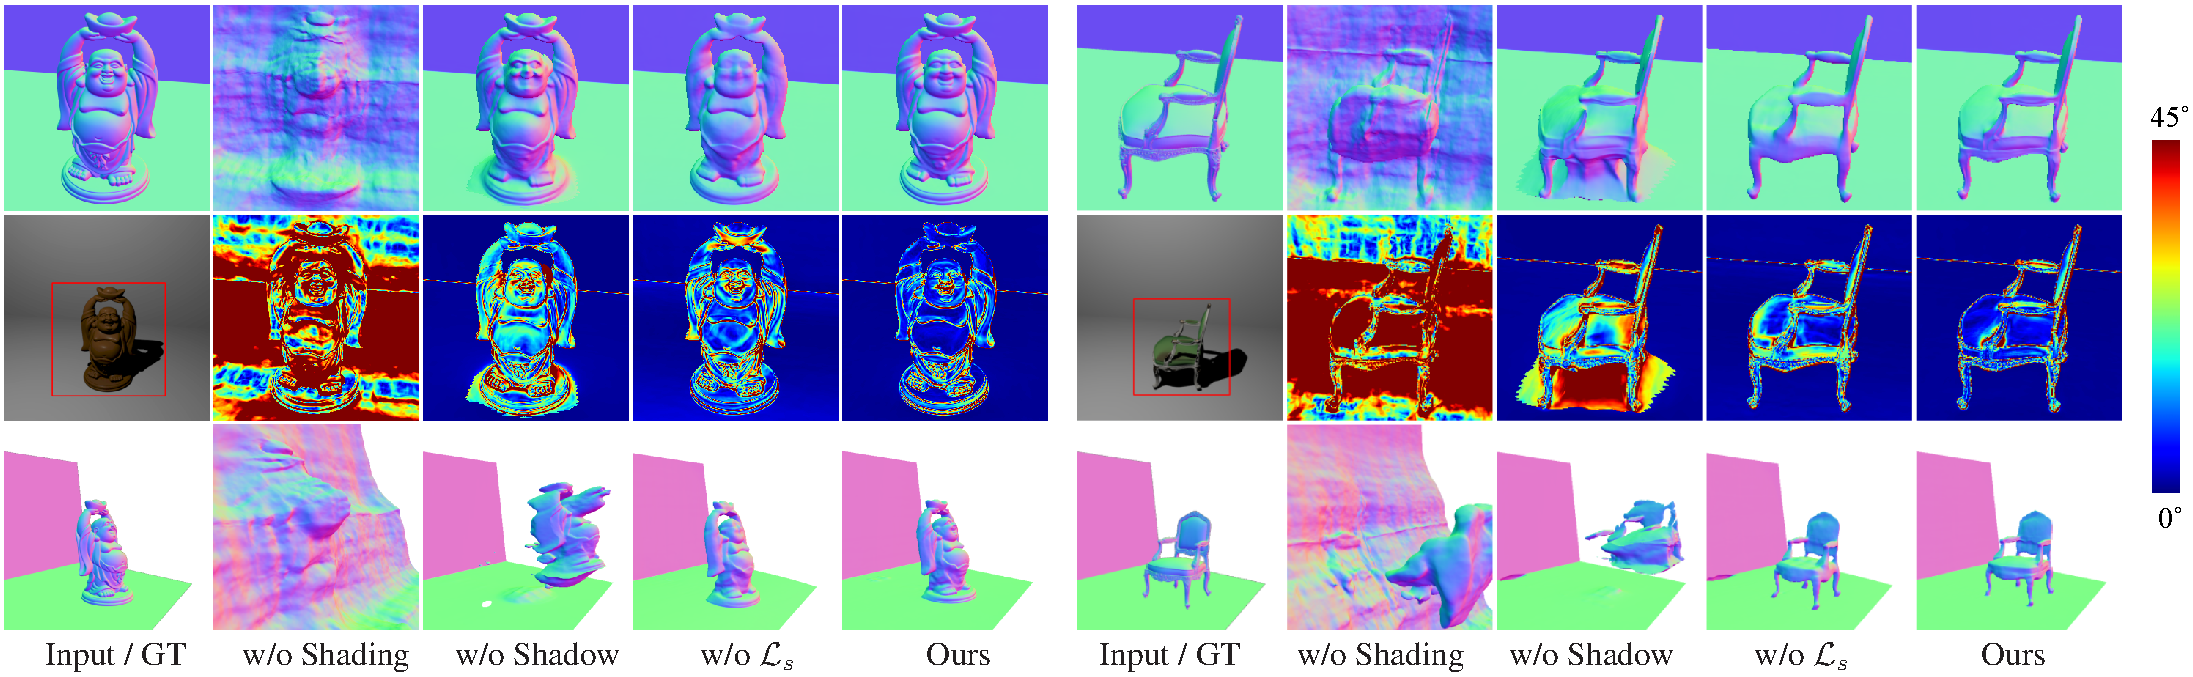
\includegraphics[align=c,width=\textwidth]{images/fig_ablation.pdf} 
        \end{center}
        
        
        \vspace{-0.3em}
        %%%%%%%%%%%%%%%%%%%%%%%% REAL  %%%%%%%%%%%%%%%%%%%%%%%%%%%%%
        \textbf{\color{ctitle}Results on Real Scenes:}
        \vspace{-0.5em}
        %%%%%%%%%%%%%%%%%%%%%%%% figure  %%%%%%%%%%%%%%%%%%%%%%%%%%%%%
        \begin{center}
            \includegraphics[align=c,width=\textwidth]{images/fig_real_case.pdf} 
        \end{center}
        
        
        %%%%%%%%%%%%%%%%%%%%%%%% Capturing Setup  %%%%%%%%%%%%%%%%%%%%%%%%%
        \def\realheight{0.22\textwidth}
        \vspace{-0.5em}
        \begin{minipage}[t]{0.58\textwidth}
        \textbf{\color{ctitle}Capturing Setup:} \\
        \vspace{-1.5em}
        \begin{center}
            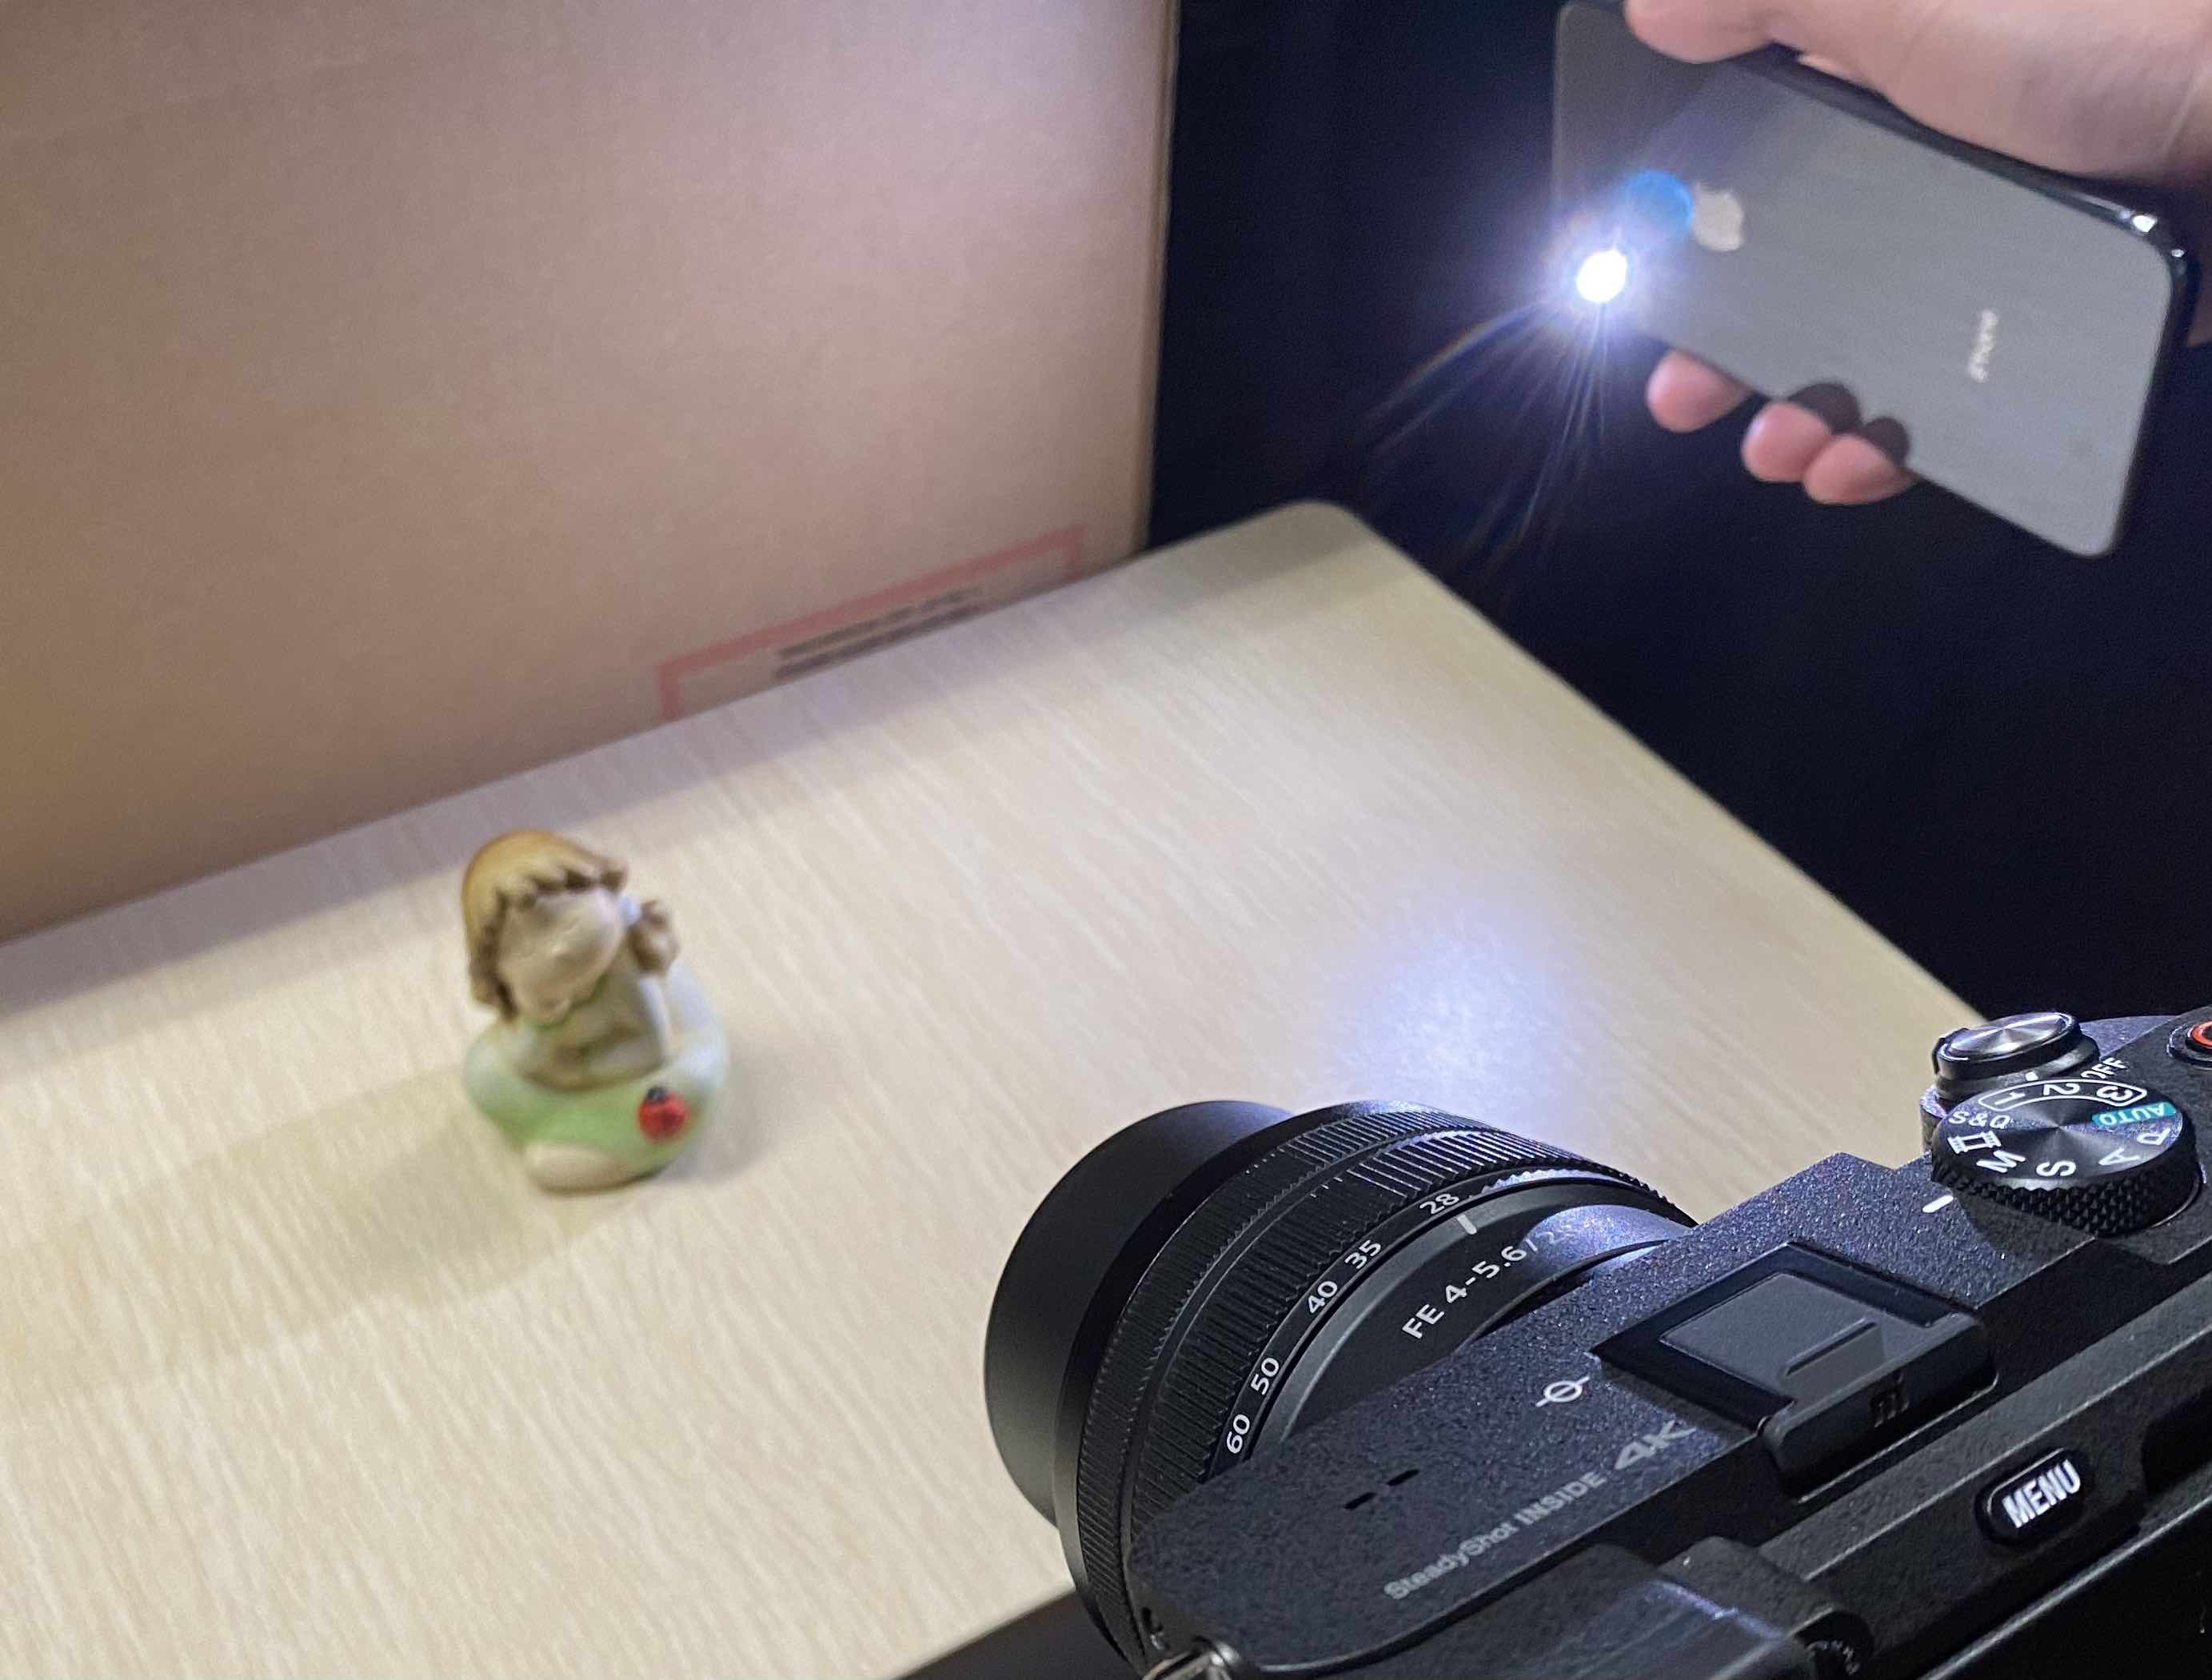
\includegraphics[align=c,height=\realheight]{images/showcase/setup.jpg}
            \hfill
            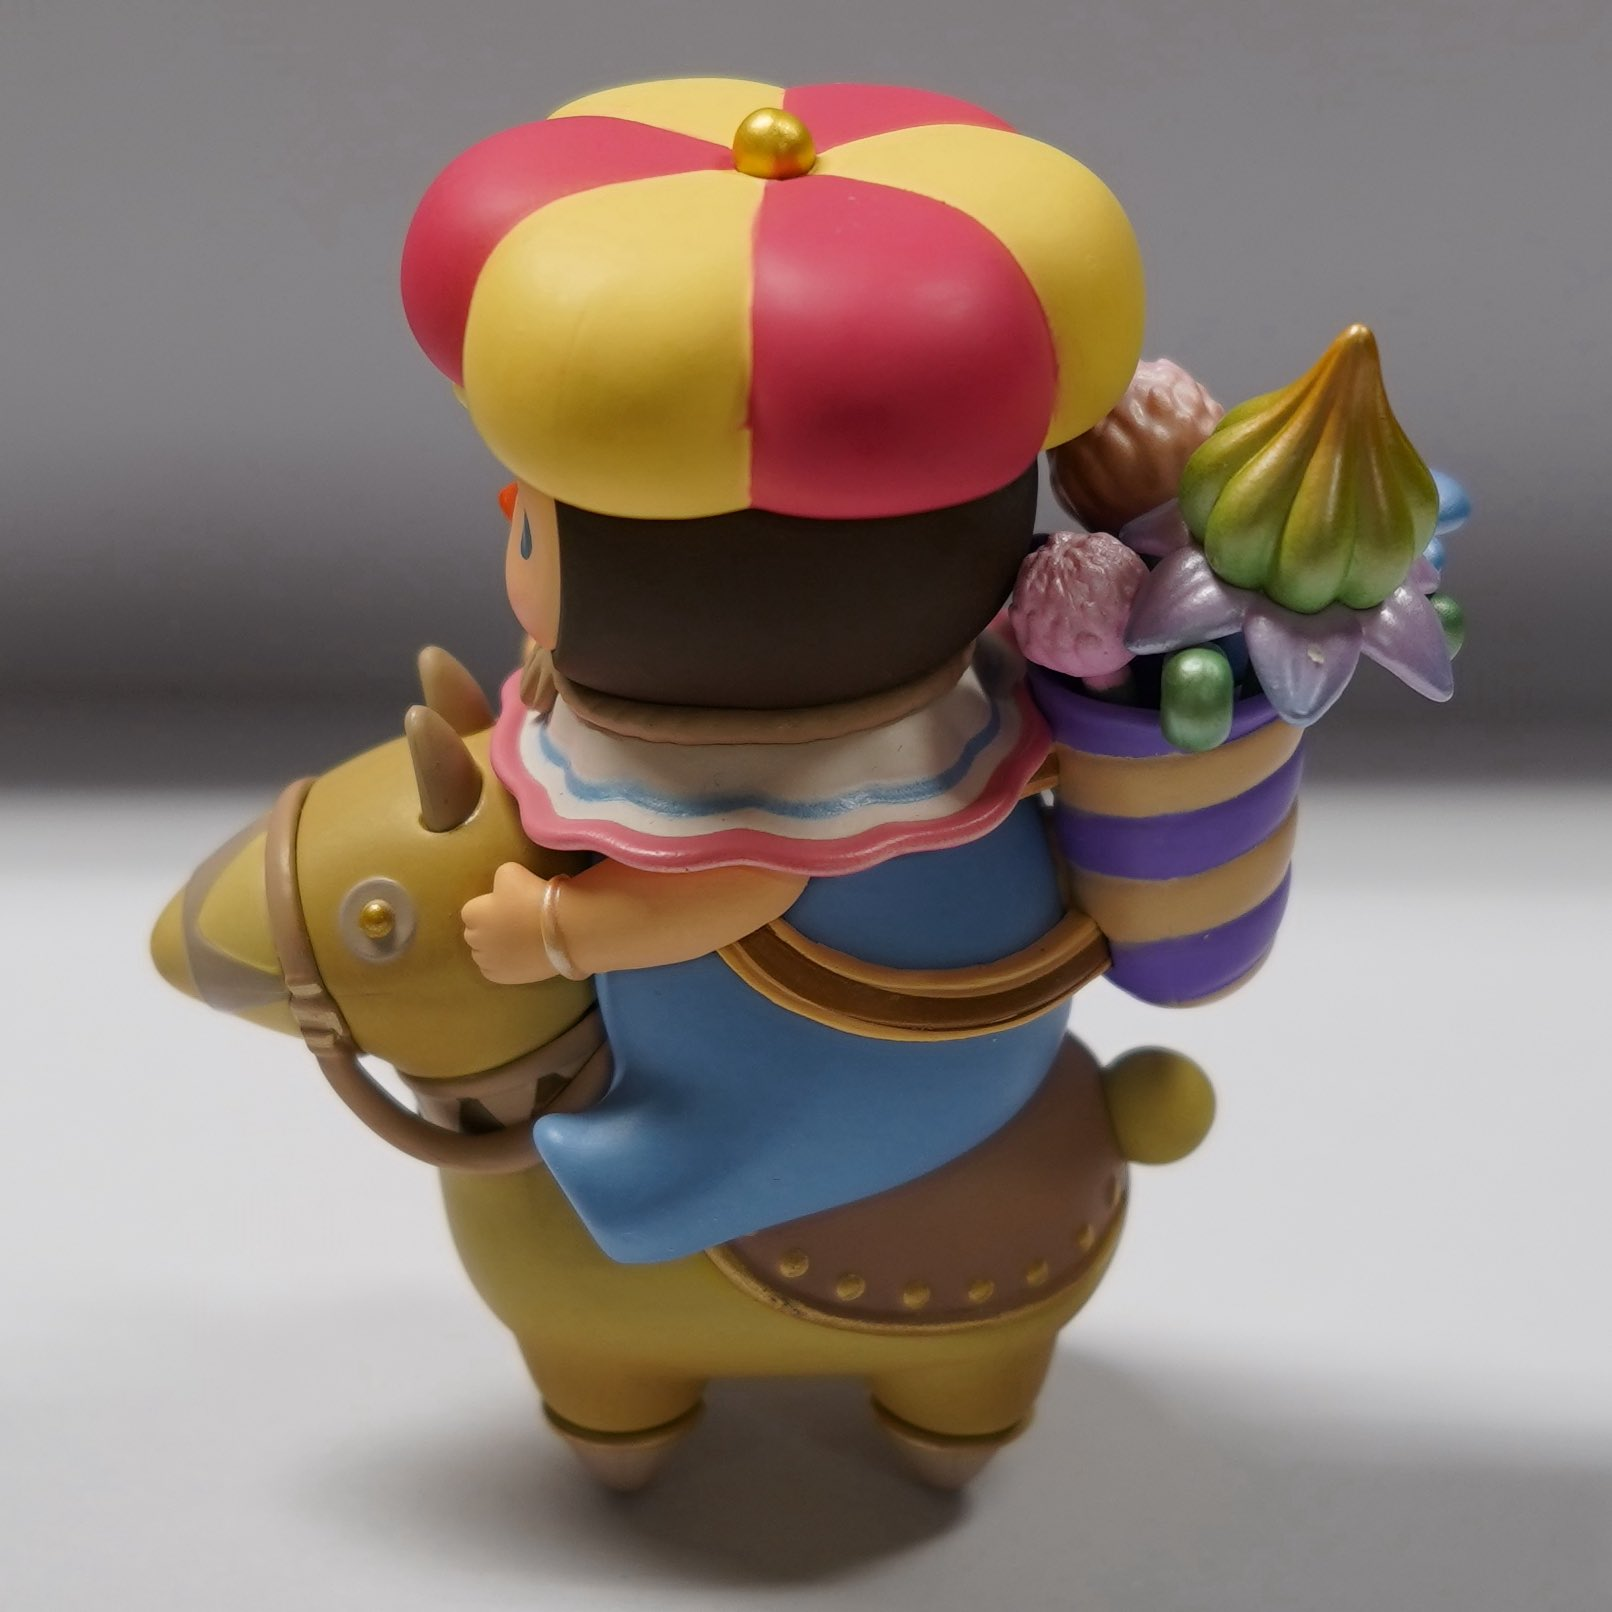
\includegraphics[align=c,height=\realheight]{images/showcase/botanist_left.jpg}
            \hfill
            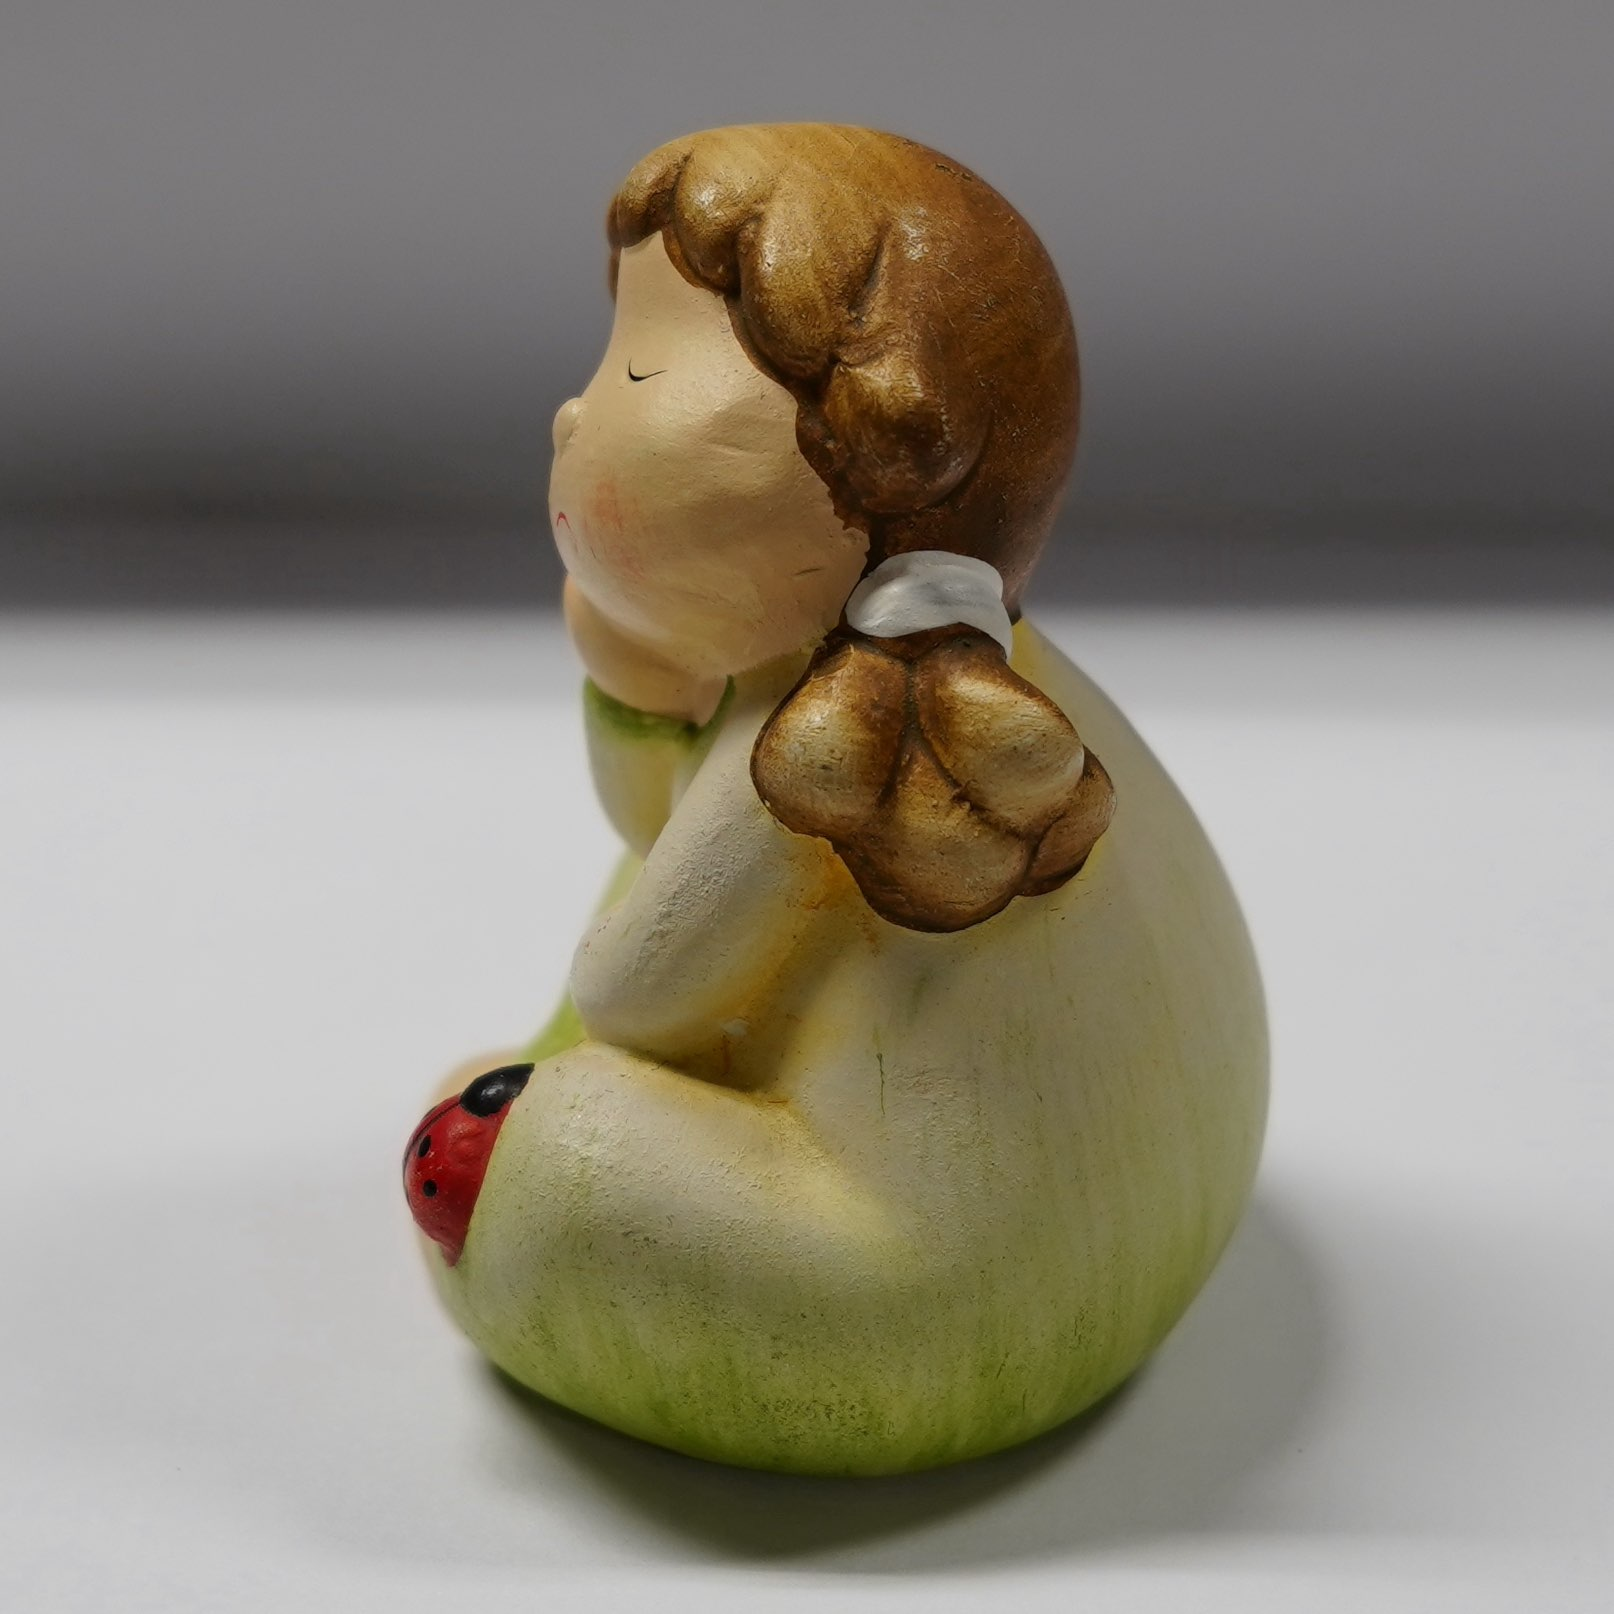
\includegraphics[align=c,height=\realheight]{images/showcase/girl_left.jpg}
            \hfill
            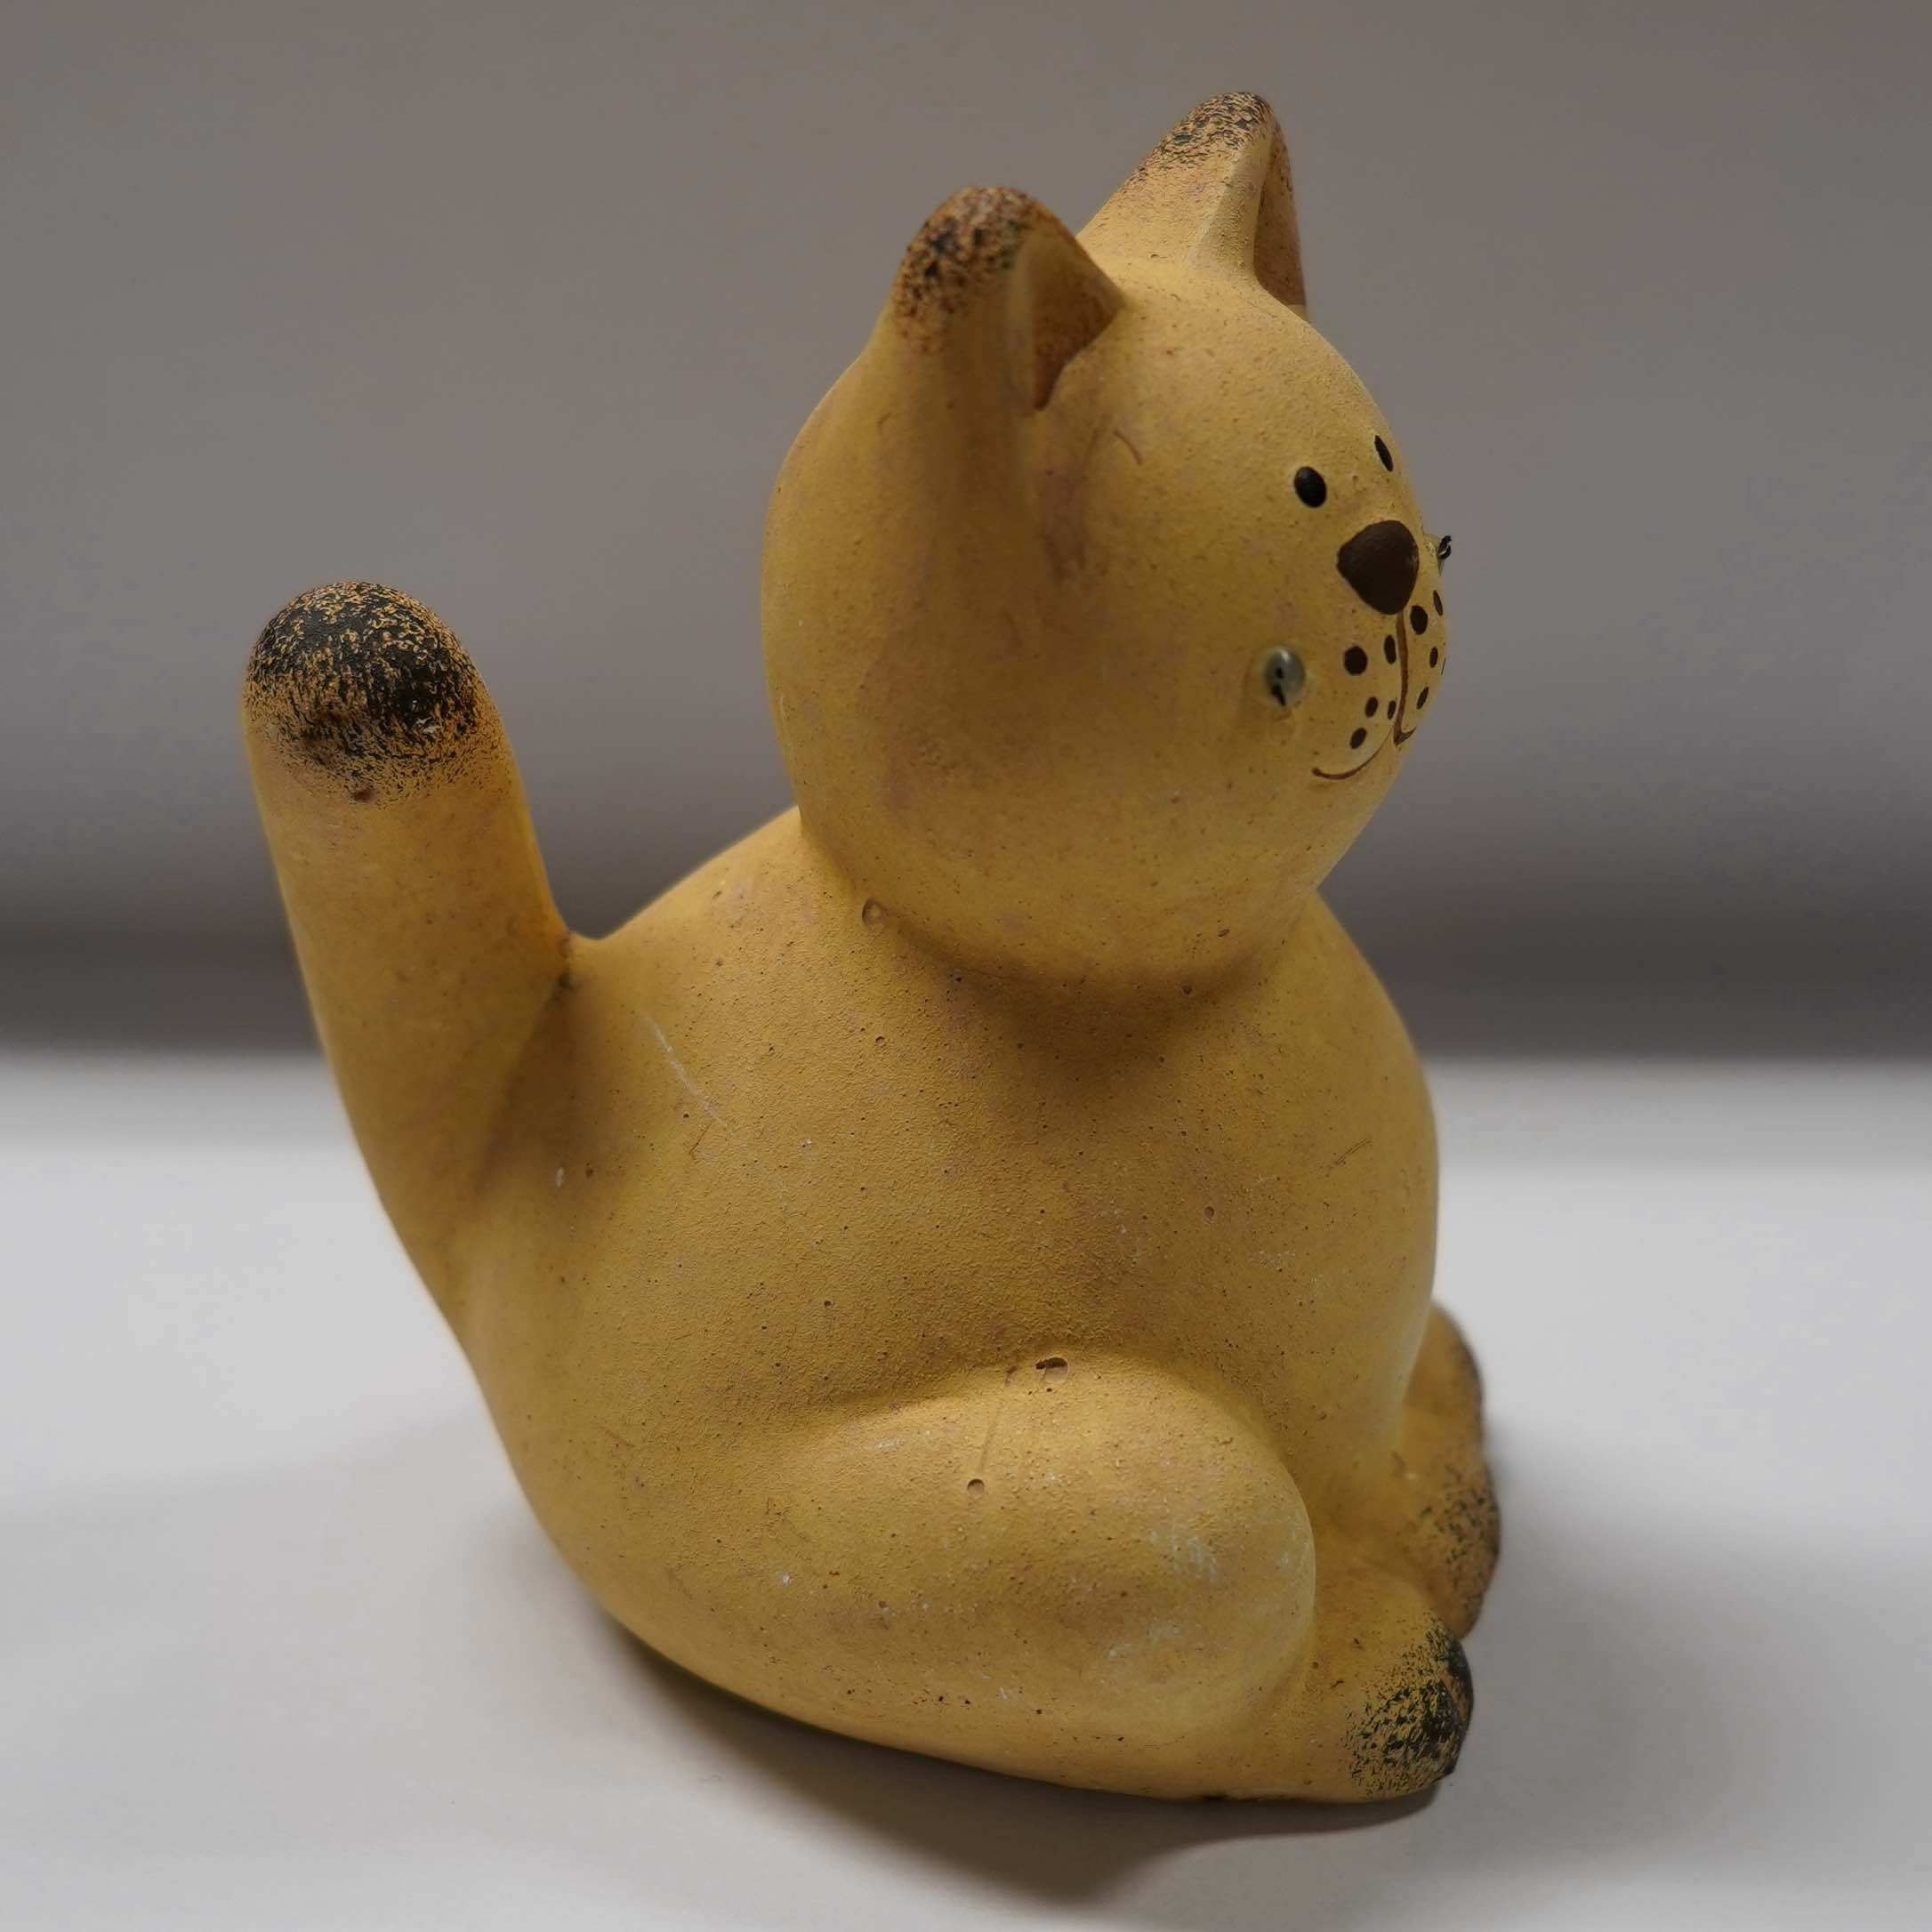
\includegraphics[align=c,height=\realheight]{images/showcase/cat_right.jpg}
        \end{center}
        \end{minipage}\hfill
        %%%%%%%%%%%%%%%%%%%%%%%% REFERENCE  %%%%%%%%%%%%%%%%%%%%%%%%%%%%%
        \begin{minipage}[t]{0.4\textwidth}
        \textbf{\color{ctitle}References:} \\
            \vspace{-0.8em}
            \begin{enumerate}[label={[\arabic*]}, leftmargin=*]
                \scriptsize
                \item NeRF [Mildenhall~\emph{et al.}, ECCV20]
                \item UNISURF [Oechsle~\emph{et al.}, ICCV21]
                \item ZL18 [Li~\emph{et al.}, TOG18]
                \item QY18 [Quéau~\emph{et al.}, JMIV18]
                \item HS20 [Santo~\emph{et al.}, ECCV20]
            \end{enumerate}
        \end{minipage}
    \end{minipage}

}
\end{poster}
\end{document}